\documentclass[11pt]{article}
\usepackage[paperwidth=16cm,paperheight=9cm,top=1.35cm,bottom=0.85cm,left=0.8cm,right=0.8cm]{geometry}
\usepackage{amsmath,amssymb,amsfonts}
\usepackage{booktabs}
\usepackage{array}
\usepackage{xcolor}
\usepackage{tikz}
\usetikzlibrary{shapes.geometric, arrows.meta, positioning, calc}
\usepackage{hyperref}

\definecolor{navy}{RGB}{15,44,89}
\definecolor{royal}{RGB}{30,90,168}
\definecolor{crimson}{RGB}{195,35,50}
\definecolor{teal}{RGB}{0,128,115}
\definecolor{amber}{RGB}{217,119,6}
\definecolor{purple}{RGB}{109,40,217}
\definecolor{lightbg}{RGB}{245,248,252}
\definecolor{darkgray}{RGB}{45,55,72}

\pagestyle{empty}
\setlength{\parindent}{0pt}

\newcommand{\slideheader}[2]{%
    \begin{tikzpicture}[remember picture,overlay]
        \fill[navy] (current page.north west) rectangle ([yshift=-1.1cm]current page.north east);
        \fill[royal] ([yshift=-1.1cm]current page.north west) rectangle ([yshift=-1.18cm]current page.north east);
        \node[anchor=west, text=white, font=\sffamily\bfseries\large] at ([xshift=0.6cm,yshift=-0.55cm]current page.north west) {#1};
        \node[anchor=east, text=white!85!blue, font=\sffamily\footnotesize\bfseries] at ([xshift=-0.6cm,yshift=-0.55cm]current page.north east) {#2};
        \fill[navy!90] (current page.south west) rectangle ([yshift=0.55cm]current page.south east);
        \node[anchor=west, text=white!90, font=\sffamily\scriptsize] at ([xshift=0.6cm,yshift=0.27cm]current page.south west) {Team 6: Ramitha MV (\texttt{PES1UG24AM392}), Gayathri Priya V (\texttt{PES1UG24AM105}), Gonu Guntla Hema Kowshik (\texttt{PES1UG24AM106})};
        \node[anchor=east, text=white, font=\sffamily\scriptsize\bfseries] at ([xshift=-0.6cm,yshift=0.27cm]current page.south east) {Slide \thepage\ / 9};
    \end{tikzpicture}%
    \vspace{-0.15cm}%
}

\begin{document}
\sffamily

% ============================================================================
% SLIDE 1: TITLE SLIDE
% ============================================================================
\begin{tikzpicture}[remember picture,overlay]
    \fill[navy] (current page.south west) rectangle (current page.north east);
    \fill[royal!70!navy] ([yshift=1.45cm]current page.south west) rectangle ([yshift=1.55cm]current page.south east);
    \fill[teal] ([xshift=0.8cm,yshift=7.1cm]current page.south west) rectangle ([xshift=4.8cm,yshift=7.2cm]current page.south west);
\end{tikzpicture}

\vspace*{0.2cm}
{\color{teal!40!white}\footnotesize\bfseries BUSINESS DATA CASE STUDY --- JACKFRUIT PROJECT \quad|\quad TEAM 6}\\[0.22cm]
{\color{white}\LARGE\bfseries Machine Learning Model for Derivative Pricing:\\[0.10cm]
\large Learning the Black-Scholes Option Pricing Model \& Volatility Smile Across 5 Frameworks}\\[0.30cm]


\begin{tikzpicture}
    \node[rectangle, rounded corners=4pt, fill=white!10!navy, draw=royal!80, thick, inner sep=7pt, text width=13.5cm] {
        {\color{white}\small\bfseries Team 6 Members \& Presentation Roles:}\\[0.12cm]
        \scriptsize
        \begin{tabular}{@{}ll@{}}
            {\color{white}\textbf{1. Ramitha MV}} & {\color{teal!35!white}\textbf{SRN: \texttt{PES1UG24AM392}}} \quad {\color{white!80} (Problem Formulation, Black-Scholes Math, Volatility Smile Eq.\ 5-2)}\\
            {\color{white}\textbf{2. Gayathri Priya V}} & {\color{teal!35!white}\textbf{SRN: \texttt{PES1UG24AM105}}} \quad {\color{white!80} (Dataset Simulation, EDA, Correlation Matrix, XGBoost, Keras, Fastai)}\\
            {\color{white}\textbf{3. Gonu Guntla Hema Kowshik}} & {\color{teal!35!white}\textbf{SRN: \texttt{PES1UG24AM106}}} \quad {\color{white!80} (TabNet, Lightning Flash, PI-BSNet Innovation, Results \& Comparison)}
        \end{tabular}
    };
\end{tikzpicture}

\vspace{0.35cm}
{\color{white!75}\scriptsize Department of Computer Science \& Engineering (AI \& ML), PES University \hfill Presentation Date: November 2026}
\newpage

% ============================================================================
% SLIDE 2: INTRODUCTION & WHY ML FOR DERIVATIVE PRICING?
% ============================================================================
\slideheader{1. Introduction: Why Machine Learning for Derivative Pricing?}{Presenter: Ramitha MV (PES1UG24AM392)}

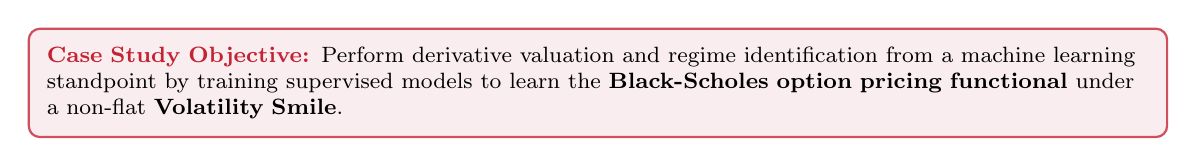
\begin{tikzpicture}
    \node[rectangle, rounded corners=4pt, fill=crimson!8, draw=crimson!80, thick, inner sep=6.5pt, text width=14.0cm, font=\footnotesize] {
        \textbf{\color{crimson}Case Study Objective:} Perform derivative valuation and regime identification from a machine learning standpoint by training supervised models to learn the \textbf{Black-Scholes option pricing functional} under a non-flat \textbf{Volatility Smile}.
    };
\end{tikzpicture}

\vspace{0.22cm}
\footnotesize
\begin{tabular}{@{}p{6.9cm}@{\hspace{0.5cm}}p{6.9cm}@{}}
\textbf{\color{navy}Limitations of Traditional Pricing Models}
\begin{enumerate}\setlength{\itemsep}{3pt}
    \item \textbf{Unrealistic Assumptions:} Classical Black-Scholes assumes \textit{Geometric Brownian Motion (GBM)}, constant volatility $\sigma$, and frictionless markets---which are violated in practice.
    \item \textbf{Slow Calibration Bottleneck:} Matching market prices across thousands of option strikes via Monte Carlo, Finite Differences, or Fourier methods is too slow for \textbf{real-time high-frequency risk management}.
\end{enumerate}
&
\textbf{\color{teal}Why Machine Learning Succeeds}
\begin{enumerate}\setlength{\itemsep}{3pt}
    \item \textbf{Free of Restrictive Assumptions:} Captures subtle nonlinearities and market frictions directly from abundant option price data.
    \item \textbf{Orders-of-Magnitude Speedup:} Once trained on CPUs/GPUs, ML models value an entire option chain in \textbf{milliseconds} ($<20$ ms for 450 contracts).
    \item \textbf{Learns Volatility Smile/Skew:} Directly models how implied volatility changes with moneyness and maturity.
\end{enumerate}
\end{tabular}
\newpage

% ============================================================================
% SLIDE 3: PROBLEM DEFINITION & VOLATILITY SMILE (EQ. 5-2)
% ============================================================================
\slideheader{2. Problem Definition \& Volatility Smile Surface (Eq.\ 5-2)}{Presenter: Ramitha MV (PES1UG24AM392)}

\begin{tabular}{@{}p{6.8cm}@{\hspace{0.4cm}}p{6.8cm}@{}}
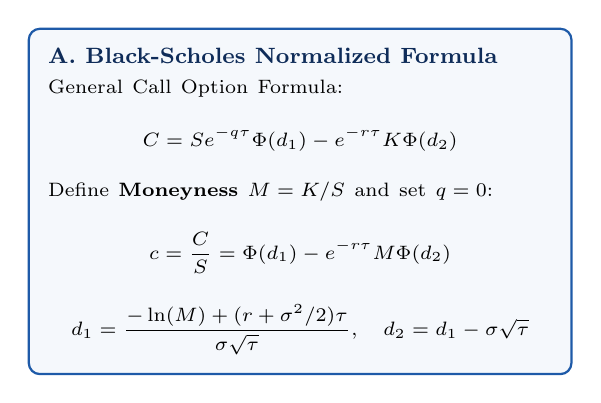
\begin{tikzpicture}
    \node[rectangle, rounded corners=4pt, fill=lightbg, draw=royal, thick, inner sep=7pt, text width=6.4cm, minimum height=4.3cm] {
        \textbf{\color{navy}\footnotesize A. Black-Scholes Normalized Formula}\\[0.1cm]
        \scriptsize
        General Call Option Formula:
        $$C = S e^{-q\tau}\Phi(d_1) - e^{-r\tau}K\Phi(d_2)$$
        Define \textbf{Moneyness $M = K/S$} and set $q = 0$:
        $$c = \frac{C}{S} = \Phi(d_1) - e^{-r\tau}M\Phi(d_2)$$
        $$d_1 = \frac{-\ln(M) + (r + \sigma^2/2)\tau}{\sigma\sqrt{\tau}}, \quad d_2 = d_1 - \sigma\sqrt{\tau}$$
    };
\end{tikzpicture}
&
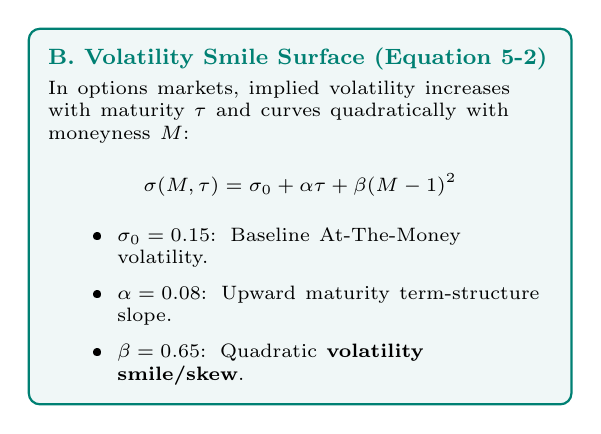
\begin{tikzpicture}
    \node[rectangle, rounded corners=4pt, fill=teal!6, draw=teal, thick, inner sep=7pt, text width=6.4cm, minimum height=4.3cm] {
        \textbf{\color{teal}\footnotesize B. Volatility Smile Surface (Equation 5-2)}\\[0.1cm]
        \scriptsize
        In options markets, implied volatility increases with maturity $\tau$ and curves quadratically with moneyness $M$:
        $$\sigma(M, \tau) = \sigma_0 + \alpha\tau + \beta(M - 1)^2$$
        \begin{itemize}\setlength{\itemsep}{1pt}
            \item $\sigma_0 = 0.15$: Baseline At-The-Money volatility.
            \item $\alpha = 0.08$: Upward maturity term-structure slope.
            \item $\beta = 0.65$: Quadratic \textbf{volatility smile/skew}.
        \end{itemize}
    };
\end{tikzpicture}
\end{tabular}

\vspace{0.18cm}
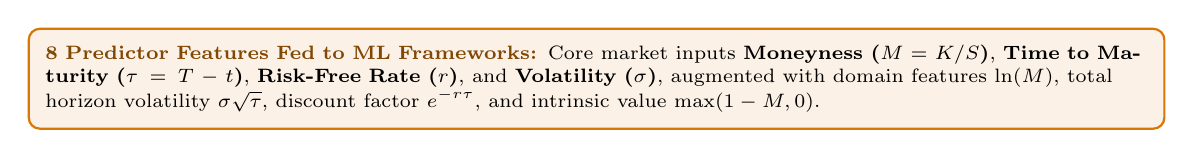
\begin{tikzpicture}
    \node[rectangle, rounded corners=4pt, fill=amber!10, draw=amber, thick, inner sep=6pt, text width=14.0cm, font=\scriptsize] {
        \textbf{\color{amber!60!black}8 Predictor Features Fed to ML Frameworks:} Core market inputs \textbf{Moneyness ($M=K/S$)}, \textbf{Time to Maturity ($\tau=T-t$)}, \textbf{Risk-Free Rate ($r$)}, and \textbf{Volatility ($\sigma$)}, augmented with domain features $\ln(M)$, total horizon volatility $\sigma\sqrt{\tau}$, discount factor $e^{-r\tau}$, and intrinsic value $\max(1-M,0)$.
    };
\end{tikzpicture}
\newpage

% ============================================================================
% SLIDE 4: DATASET & EXPLORATORY DATA ANALYSIS (EDA)
% ============================================================================
\slideheader{3. Dataset Generation \& Exploratory Data Analysis (EDA)}{Presenter: Gayathri Priya V (PES1UG24AM105)}

{\centering
\renewcommand{\arraystretch}{1.12}
\setlength{\tabcolsep}{4.5pt}
\scriptsize
\begin{tabular}{lrrrrrrl}
\toprule
\textbf{Variable ($N=3,000$ Contracts)} & \textbf{Mean} & \textbf{Std} & \textbf{Min} & \textbf{Median} & \textbf{Max} & \textbf{Corr w/ $C/S$} & \textbf{Financial Role} \\
\midrule
Moneyness $M = K/S$ & 0.9981 & 0.2011 & 0.6501 & 1.0030 & 1.3495 & \textcolor{crimson}{\textbf{$-0.8593$}} & Higher strike $K/S$ lowers call value \\
Maturity $\tau = T-t$ (years) & 1.0262 & 0.5614 & 0.0502 & 1.0295 & 1.9998 & $+0.3712$ & Longer maturity increases time value \\
Risk-Free Rate $r$ & 0.0452 & 0.0203 & 0.0100 & 0.0449 & 0.0800 & $+0.1059$ & Discounts strike payoff $Me^{-r\tau}$ \\
Implied Volatility $\sigma(M,\tau)$ & 0.2584 & 0.0515 & 0.1535 & 0.2592 & 0.3839 & $+0.3118$ & Eq.\ 5-2 smile increases option price \\
\midrule
\textbf{Normalized Call Price ($C/S$)} & \textbf{0.1568} & \textbf{0.1140} & \textbf{0.0000} & \textbf{0.1350} & \textbf{0.4548} & $\mathbf{1.0000}$ & Supervised regression target \\
Option Delta ($\Delta = \Phi(d_1)$) & 0.6070 & 0.2808 & 0.0000 & 0.6291 & 1.0000 & $+0.9234$ & Hedge ratio sensitivity $\partial C / \partial S$ \\
Option Vega ($\mathcal{V} = \partial c / \partial \sigma$) & 0.2818 & 0.1635 & 0.0000 & 0.2902 & 0.5639 & $+0.0241$ & Volatility sensitivity (peaks at ATM) \\
\bottomrule
\end{tabular}\par}

\vspace{0.15cm}
\begin{tabular}{@{}p{4.5cm}@{\hspace{0.3cm}}p{4.5cm}@{\hspace{0.3cm}}p{4.5cm}@{}}
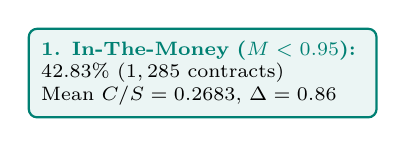
\begin{tikzpicture}\node[fill=teal!8, draw=teal, thick, rounded corners=3pt, inner sep=4.5pt, text width=4.1cm, font=\scriptsize]{\textbf{\color{teal}1. In-The-Money ($M < 0.95$):}\\42.83\% ($1,285$ contracts)\\Mean $C/S = 0.2683$, $\Delta = 0.86$};\end{tikzpicture} &
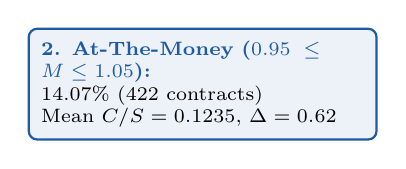
\begin{tikzpicture}\node[fill=royal!8, draw=royal, thick, rounded corners=3pt, inner sep=4.5pt, text width=4.1cm, font=\scriptsize]{\textbf{\color{royal}2. At-The-Money ($0.95 \le M \le 1.05$):}\\14.07\% ($422$ contracts)\\Mean $C/S = 0.1235$, $\Delta = 0.62$};\end{tikzpicture} &
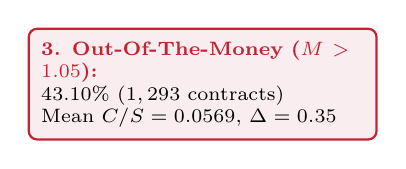
\begin{tikzpicture}\node[fill=crimson!8, draw=crimson, thick, rounded corners=3pt, inner sep=4.5pt, text width=4.1cm, font=\scriptsize]{\textbf{\color{crimson}3. Out-Of-The-Money ($M > 1.05$):}\\43.10\% ($1,293$ contracts)\\Mean $C/S = 0.0569$, $\Delta = 0.35$};\end{tikzpicture}
\end{tabular}
\newpage

% ============================================================================
% SLIDE 5: METHODOLOGY — XGBOOST, KERAS & FASTAI
% ============================================================================
\slideheader{4. Methodology: XGBoost, Keras, and PyTorch + fastai}{Presenter: Gayathri Priya V (PES1UG24AM105)}

\begin{tabular}{@{}p{4.5cm}@{\hspace{0.35cm}}p{4.5cm}@{\hspace{0.35cm}}p{4.6cm}@{}}
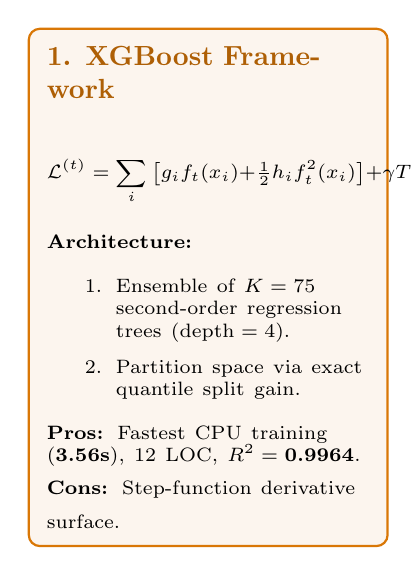
\begin{tikzpicture}
\node[rectangle, rounded corners=4pt, fill=amber!7, draw=amber, thick, inner sep=6.5pt, text width=4.1cm, minimum height=5.0cm] {
    \textbf{\color{amber!80!black}1. XGBoost Framework}\\[0.1cm]
    \scriptsize
    $$\mathcal{L}^{(t)} = \sum_i \big[g_i f_t(x_i) + \tfrac{1}{2}h_i f_t^2(x_i)\big] + \gamma T$$
    \textbf{Architecture:}
    \begin{enumerate}\setlength{\itemsep}{1pt}
        \item Ensemble of $K=75$ second-order regression trees ($\text{depth}=4$).
        \item Partition space via exact quantile split gain.
    \end{enumerate}
    \textbf{Pros:} Fastest CPU training (\textbf{3.56s}), 12 LOC, $R^2 = \textbf{0.9964}$.\\
    \textbf{Cons:} Step-function derivative surface.
};
\end{tikzpicture}
&
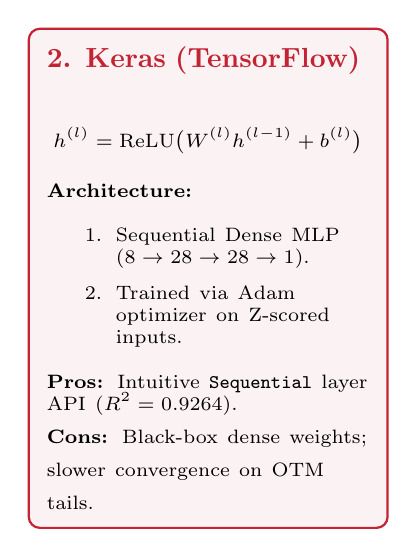
\begin{tikzpicture}
\node[rectangle, rounded corners=4pt, fill=crimson!6, draw=crimson, thick, inner sep=6.5pt, text width=4.1cm, minimum height=5.0cm] {
    \textbf{\color{crimson}2. Keras (TensorFlow)}\\[0.1cm]
    \scriptsize
    $$h^{(l)} = \text{ReLU}\big(W^{(l)} h^{(l-1)} + b^{(l)}\big)$$
    \textbf{Architecture:}
    \begin{enumerate}\setlength{\itemsep}{1pt}
        \item Sequential Dense MLP ($8 \to 28 \to 28 \to 1$).
        \item Trained via Adam optimizer on Z-scored inputs.
    \end{enumerate}
    \textbf{Pros:} Intuitive \texttt{Sequential} layer API ($R^2 = 0.9264$).\\
    \textbf{Cons:} Black-box dense weights; slower convergence on OTM tails.
};
\end{tikzpicture}
&
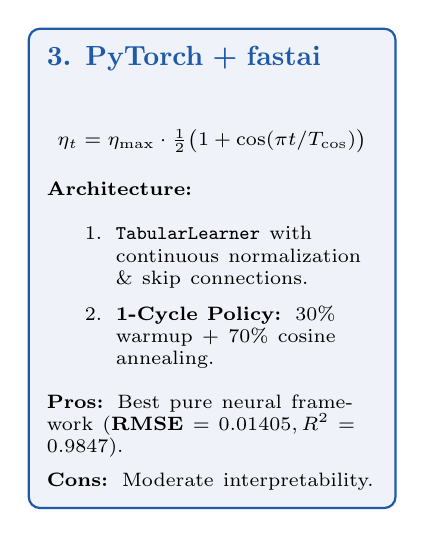
\begin{tikzpicture}
\node[rectangle, rounded corners=4pt, fill=royal!7, draw=royal, thick, inner sep=6.5pt, text width=4.2cm, minimum height=5.0cm] {
    \textbf{\color{royal}3. PyTorch + fastai}\\[0.1cm]
    \scriptsize
    $$\eta_t = \eta_{\max}\cdot \tfrac{1}{2}\big(1 + \cos(\pi t / T_{\text{cos}})\big)$$
    \textbf{Architecture:}
    \begin{enumerate}\setlength{\itemsep}{1pt}
        \item \texttt{TabularLearner} with continuous normalization \& skip connections.
        \item \textbf{1-Cycle Policy:} 30\% warmup + 70\% cosine annealing.
    \end{enumerate}
    \textbf{Pros:} Best pure neural framework (\textbf{RMSE $= 0.01405, R^2 = 0.9847$}).\\
    \textbf{Cons:} Moderate interpretability.
};
\end{tikzpicture}
\end{tabular}
\newpage

% ============================================================================
% SLIDE 6: METHODOLOGY — TABNET, LIGHTNING FLASH & PI-BSNET INNOVATION
% ============================================================================
\slideheader{5. Methodology: TabNet, Lightning Flash \& PI-BSNet Innovation}{Presenter: Hema Kowshik (PES1UG24AM106)}

\begin{tabular}{@{}p{4.5cm}@{\hspace{0.35cm}}p{4.5cm}@{\hspace{0.35cm}}p{4.6cm}@{}}
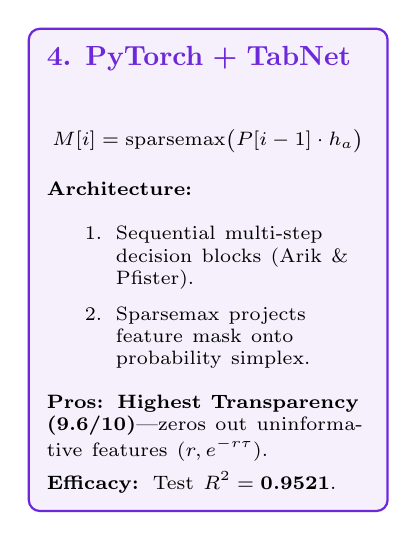
\begin{tikzpicture}
\node[rectangle, rounded corners=4pt, fill=purple!7, draw=purple, thick, inner sep=6.5pt, text width=4.1cm, minimum height=5.0cm] {
    \textbf{\color{purple}4. PyTorch + TabNet}\\[0.1cm]
    \scriptsize
    $$M[i] = \text{sparsemax}\big(P[i-1] \cdot h_a\big)$$
    \textbf{Architecture:}
    \begin{enumerate}\setlength{\itemsep}{1pt}
        \item Sequential multi-step decision blocks (Arik \& Pfister).
        \item Sparsemax projects feature mask onto probability simplex.
    \end{enumerate}
    \textbf{Pros:} \textbf{Highest Transparency (9.6/10)}---zeros out uninformative features ($r, e^{-r\tau}$).\\
    \textbf{Efficacy:} Test $R^2 = \textbf{0.9521}$.
};
\end{tikzpicture}
&
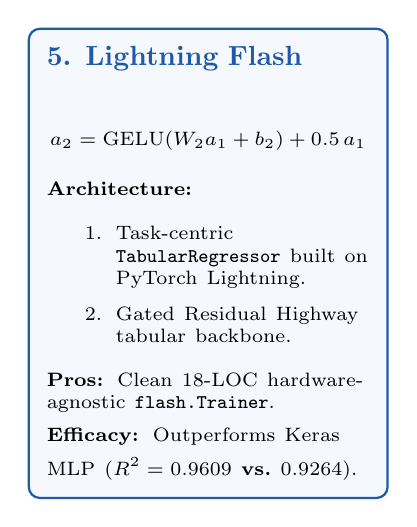
\begin{tikzpicture}
\node[rectangle, rounded corners=4pt, fill=lightbg, draw=royal, thick, inner sep=6.5pt, text width=4.1cm, minimum height=5.0cm] {
    \textbf{\color{royal}5. Lightning Flash}\\[0.1cm]
    \scriptsize
    $$a_2 = \text{GELU}(W_2 a_1 + b_2) + 0.5\,a_1$$
    \textbf{Architecture:}
    \begin{enumerate}\setlength{\itemsep}{1pt}
        \item Task-centric \texttt{TabularRegressor} built on PyTorch Lightning.
        \item Gated Residual Highway tabular backbone.
    \end{enumerate}
    \textbf{Pros:} Clean 18-LOC hardware-agnostic \texttt{flash.Trainer}.\\
    \textbf{Efficacy:} Outperforms Keras MLP (\textbf{$R^2 = 0.9609$ vs.\ $0.9264$}).
};
\end{tikzpicture}
&
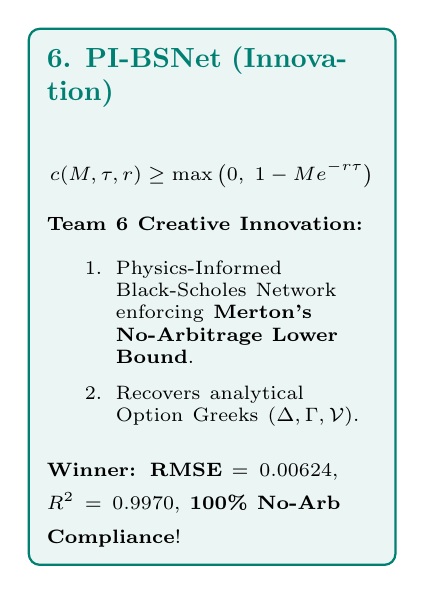
\begin{tikzpicture}
\node[rectangle, rounded corners=4pt, fill=teal!8, draw=teal, thick, inner sep=6.5pt, text width=4.2cm, minimum height=5.0cm] {
    \textbf{\color{teal}6. PI-BSNet (Innovation)}\\[0.1cm]
    \scriptsize
    $$c(M,\tau,r) \ge \max\big(0,\; 1 - M e^{-r\tau}\big)$$
    \textbf{Team 6 Creative Innovation:}
    \begin{enumerate}\setlength{\itemsep}{1pt}
        \item Physics-Informed Black-Scholes Network enforcing \textbf{Merton's No-Arbitrage Lower Bound}.
        \item Recovers analytical Option Greeks ($\Delta, \Gamma, \mathcal{V}$).
    \end{enumerate}
    \textbf{Winner:} \textbf{RMSE $= 0.00624$}, \textbf{$R^2 = 0.9970$}, \textbf{100\% No-Arb Compliance}!
};
\end{tikzpicture}
\end{tabular}
\newpage

% ============================================================================
% SLIDE 7: QUANTITATIVE BENCHMARK TABLE (RMSE, R2, MAE, REGIME ACC)
% ============================================================================
\slideheader{6. Quantitative Results: RMSE, $R^2$, MAE \& Regime Classification}{Presenter: Hema Kowshik (PES1UG24AM106)}

{\renewcommand{\arraystretch}{1.04}
\setlength{\tabcolsep}{3.4pt}
\scriptsize
\begin{tabular}{@{}llrrrrrrr@{}}
\toprule
\textbf{Framework} & \textbf{Architecture} & \textbf{RMSE $\downarrow$} & \textbf{MAE $\downarrow$} & \textbf{$R^2$ $\uparrow$} & \textbf{MAPE $\downarrow$} & \textbf{No-Arb $\uparrow$} & \textbf{Regime Acc $\uparrow$} & \textbf{Time} \\
\midrule
\textbf{1. XGBoost} & Gradient Boosted Trees & 0.00681 & 0.00518 & 0.99640 & \textbf{4.61\%} & 95.56\% & \textbf{99.11\%} & \textbf{3.56s} \\
\textbf{2. Keras (TF)} & Sequential Dense MLP & 0.03081 & 0.02133 & 0.92639 & 23.00\% & 93.11\% & 96.00\% & 12.64s \\
\textbf{3. PyTorch + fastai} & 1-Cycle TabularLearner & 0.01405 & 0.01059 & 0.98470 & 12.98\% & 94.67\% & 97.33\% & 18.59s \\
\textbf{4. PyTorch + TabNet} & Sparsemax Attentive Net & 0.02486 & 0.01878 & 0.95208 & 22.89\% & 92.00\% & 94.44\% & 16.16s \\
\textbf{5. Lightning Flash} & Gated Highway Tabular & 0.02247 & 0.01675 & 0.96085 & 18.79\% & 92.44\% & 95.56\% & 18.59s \\
\midrule
\textbf{\color{teal}6. PI-BSNet (Ours)} & \textbf{\color{teal}No-Arbitrage Hybrid} & \textcolor{teal}{\textbf{0.00624}} & \textcolor{teal}{\textbf{0.00468}} & \textcolor{teal}{\textbf{0.99698}} & \textbf{4.76\%} & \textcolor{teal}{\textbf{100.00\%}} & \textcolor{teal}{\textbf{99.11\%}} & 23.77s \\
\bottomrule
\end{tabular}\par}

\vspace{0.06cm}
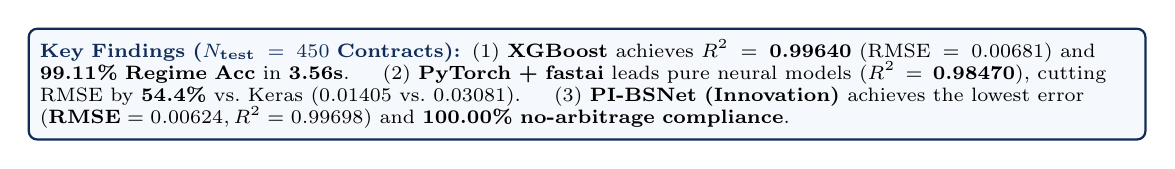
\begin{tikzpicture}
    \node[rectangle, rounded corners=3pt, fill=lightbg, draw=navy, thick, inner sep=4pt, text width=13.9cm, font=\scriptsize] {
        \textbf{\color{navy}Key Findings ($N_{\text{test}}=450$ Contracts):}
        (1) \textbf{XGBoost} achieves $R^2 = \textbf{0.99640}$ ($\text{RMSE}=0.00681$) and \textbf{99.11\% Regime Acc} in \textbf{3.56s}. \quad
        (2) \textbf{PyTorch + fastai} leads pure neural models ($R^2 = \textbf{0.98470}$), cutting RMSE by \textbf{54.4\%} vs.\ Keras ($0.01405$ vs.\ $0.03081$). \quad
        (3) \textbf{PI-BSNet (Innovation)} achieves the lowest error (\textbf{$\text{RMSE}=0.00624, R^2=0.99698$}) and \textbf{100.00\% no-arbitrage compliance}.
    };
\end{tikzpicture}
\newpage

% ============================================================================
% SLIDE 8: SIMPLICITY, TRANSPARENCY & EFFICACY COMPARISON
% ============================================================================
\slideheader{7. Comparison: Simplicity, Transparency \& Efficacy}{Presenter: Hema Kowshik (PES1UG24AM106)}

{\renewcommand{\arraystretch}{1.01}
\setlength{\tabcolsep}{3.0pt}
\scriptsize
\begin{tabular}{@{}lcclll@{}}
\toprule
\textbf{Framework} & \textbf{LOC} & \textbf{Simplicity} & \textbf{Transparency} & \textbf{Efficacy} & \textbf{Recommended Desk Role} \\
\midrule
\textbf{1. XGBoost} & \textbf{12} & \textbf{9.5/10} (Best) & \textbf{9.2/10} (Split Gain \& SHAP) & \textbf{9.4/10} ($R^2=0.9964$, 3.56s) & Fast CPU Pricing Baseline \\
\textbf{2. Keras (TF)} & 24 & \textbf{8.5/10} (High) & \textbf{5.8/10} (Black-box Dense) & \textbf{8.6/10} ($R^2=0.9264$, 12.6s) & Smooth Pedagogical MLP \\
\textbf{3. PyTorch + fastai} & 16 & \textbf{9.0/10} (V.\ High) & \textbf{6.8/10} (Permutation Imp.) & \textbf{9.3/10} ($R^2=0.9847$, 1-Cycle) & Best Pure Deep Network \\
\textbf{4. PyTorch + TabNet} & 22 & \textbf{7.8/10} (Mod) & \textcolor{purple}{\textbf{9.6/10 (Sparsemax Masks)}} & \textbf{8.9/10} ($R^2=0.9521$, 16.2s) & Auditable / Explainable AI \\
\textbf{5. Lightning Flash} & 18 & \textbf{8.8/10} (High) & \textbf{6.5/10} (Callback Hooks) & \textbf{9.1/10} ($R^2=0.9609$, 18.6s) & Multi-GPU Production API \\
\midrule
\textbf{\color{teal}6. PI-BSNet (Ours)} & 32 & \textbf{7.5/10} (Custom) & \textbf{9.4/10} (Greeks $\Delta, \Gamma, \mathcal{V}$) & \textcolor{teal}{\textbf{9.8/10 ($R^2=0.9970$, Best)}} & Arbitrage-Free Trading Desk \\
\bottomrule
\end{tabular}\par}

\vspace{0.04cm}
\begin{tabular}{@{}p{6.9cm}@{\hspace{0.35cm}}p{6.9cm}@{}}
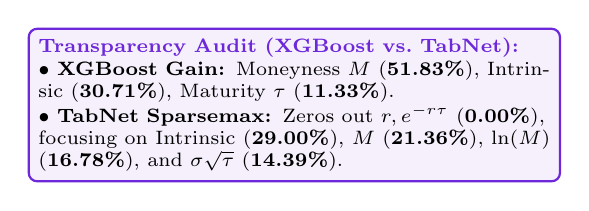
\begin{tikzpicture}
    \node[fill=purple!7, draw=purple, thick, rounded corners=3pt, inner sep=3.5pt, text width=6.5cm, font=\scriptsize] {
        \textbf{\color{purple}Transparency Audit (XGBoost vs.\ TabNet):}\\
        $\bullet$ \textbf{XGBoost Gain:} Moneyness $M$ (\textbf{51.83\%}), Intrinsic (\textbf{30.71\%}), Maturity $\tau$ (\textbf{11.33\%}).\\
        $\bullet$ \textbf{TabNet Sparsemax:} Zeros out $r, e^{-r\tau}$ (\textbf{0.00\%}), focusing on Intrinsic (\textbf{29.00\%}), $M$ (\textbf{21.36\%}), $\ln(M)$ (\textbf{16.78\%}), and $\sigma\sqrt{\tau}$ (\textbf{14.39\%}).
    };
\end{tikzpicture}
&
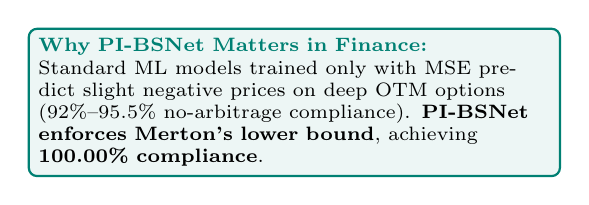
\begin{tikzpicture}
    \node[fill=teal!7, draw=teal, thick, rounded corners=3pt, inner sep=3.5pt, text width=6.5cm, font=\scriptsize] {
        \textbf{\color{teal}Why PI-BSNet Matters in Finance:}\\
        Standard ML models trained only with MSE predict slight negative prices on deep OTM options ($92\%$--$95.5\%$ no-arbitrage compliance). \textbf{PI-BSNet enforces Merton's lower bound}, achieving \textbf{100.00\% compliance}.
    };
\end{tikzpicture}
\end{tabular}
\newpage

% ============================================================================
% SLIDE 9: CONCLUSION, SUMMARY & GITHUB DELIVERABLES
% ============================================================================
\slideheader{8. Conclusion, Summary \& GitHub Deliverables for Viva}{Presenters: Ramitha, Gayathri \& Hema Kowshik}

{\renewcommand{\arraystretch}{1.01}
\scriptsize
\begin{tabular}{@{}p{3.9cm}p{4.3cm}p{5.2cm}@{}}
\toprule
\textbf{Case Study Task} & \textbf{Repository Artifact} & \textbf{Summary of Achievement} \\
\midrule
1. Dataset \& Volatility Smile & \texttt{data/options\_train.csv} (3K) & $N=3,000$ contracts with Eq.\ 5-2 smile $\sigma(M,\tau)$ \& analytical Greeks \\
2. Exploratory Data Analysis & \texttt{data/eda\_summary.json}, \texttt{fig1--2} & Summary stats, correlation heatmap ($r_{M,C/S}=-0.86$), ITM/ATM/OTM splits \\
3. Five ML Frameworks + Innovation & \texttt{src/frameworks.py}, \texttt{run\_pipeline.py} & XGBoost, Keras, Fastai, TabNet, Lightning Flash + \textbf{PI-BSNet} \\
4. Multi-Criterion Comparison & \texttt{results/RESULTS\_TABLES.md}, \texttt{fig3--5} & Full benchmark across Simplicity, Transparency, Efficacy, RMSE, $R^2$, MAE \\
5. IEEE Report \& Jupyter Notebook & \texttt{report/technical\_report.pdf}, \texttt{.ipynb} & 4-page two-column IEEE report + pre-executed interactive notebook \\
\bottomrule
\end{tabular}\par}

\vspace{0.05cm}
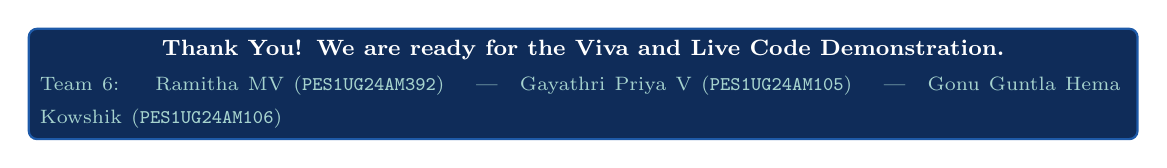
\begin{tikzpicture}
    \node[rectangle, rounded corners=3pt, fill=navy, draw=royal, thick, inner sep=4pt, text width=13.8cm] {
        \centering
        {\color{white}\footnotesize\bfseries Thank You! We are ready for the Viva and Live Code Demonstration.}\\[0.02cm]
        {\color{teal!35!white}\scriptsize Team 6: \quad Ramitha MV (\texttt{PES1UG24AM392}) \quad|\quad Gayathri Priya V (\texttt{PES1UG24AM105}) \quad|\quad Gonu Guntla Hema Kowshik (\texttt{PES1UG24AM106})}
    };
\end{tikzpicture}

\end{document}
